% GUIDA VELOCE:
% --------------------------------------------------------------------
% X INIZIA UN UNOVO CAPITOLO:
% \chapter{??? NOME CAPITOLO}}
% \section{ ?? }
% \subsection{ ?? }
%
% --------------------------------------------------------------------
% PAROLA CONTENUTA NEL GLOSSARIO:
% scrivere la parola seguita da $^g$
% esempio: User$^g$
%
% --------------------------------------------------------------------
% PER ANDARE A CAPO SENZA RIENTRO INSERIRE:
% \\
%
% --------------------------------------------------------------------
% GRASSETO:
% \textbf{parola}
%
% --------------------------------------------------------------------
% CORSIVO:
% \emph{parola}
% --------------------------------------------------------------------
% PER SCRIVERE IN ROSSO:
% \red{parola}
%
% --------------------------------------------------------------------
% PER SCRIVERE TRA VIRGOLETTE
% ''parola''
%
% --------------------------------------------------------------------
% PER EVITARE IL RIENTRO AUTOMATICO DI UN CAPOVERSO:
% \noindent testo....
%
% --------------------------------------------------------------------

% PER SCRIVERE CARATTERI PARTICOLARI COME: { } _ ecc.. SCRIVERLI PRECEDUTI DA \
% ES: \{ \_
%
% --------------------------------------------------------------------
% X INSERIRE UN LINK:
% \url{http://www.math.unipd.it/~tullio/IS-1/2011/Progetto/C3.pdf}
%
% --------------------------------------------------------------------
% PER COMMENTARE INTERE PARTI:
% \comment{ comment }
%
% --------------------------------------------------------------------
% PER SCRIVERE NOTE DURANTE IL TESTO:
% parola \footnote{ note riguardanti la parola }
%
% --------------------------------------------------------------------
% PER SCRIVERE CODICE SORGENTE:
%
% \lstset{language=c++,
% stringstyle=\color{blue}\textrm,
% commentstyle=\rmfamily, numbers= none}

% \begin{lstlisting}
% CODICE
% \end{lstlisting}
%
% --------------------------------------------------------------------
% !!!!!!!! PER COSE + COMPLESSE VEDI: !!!!!!!!!!!!!!!!!!!!!!!
% !!!!!!!! PMAC/latex/GUIDA LATEX!!!.tex !!!!!!!!!!!!!!!!!!!!!!!

% per tutto il resto chiedi a lory prima di fare/scrivere cazzate !!!!!!!!!!



\documentclass[10pt,a4paper]{article}

\usepackage[italian]{babel}
\usepackage[T1]{fontenc}
\usepackage[utf8x]{inputenc} % uso utf8x xk x linux, mentre latin1 è per windows
\usepackage{lmodern} %insieme di font molto completo consigliato da LatexFacile pg13 in basso
\usepackage{microtype} %migliora riempimento delle righe. vedi LatexImpaziente pg41
%attiva il rientro di ogni prima riga di ogni sezione: capitolo,paragrafo ecc. vd LatexImpaziente pg41
\usepackage{indentfirst}
\usepackage{graphicx} % per inseire immagini
\usepackage[usenames,dvipsnames]{color}
\usepackage{lastpage} %serve per poter scrivere page 1 of N
% setta i bordi della pagina: dx e sx 3.2cm di rientro + nel lato di rilagatura rientra di altri 0mm
\usepackage[a4paper,top=3cm,bottom=3cm,left=3.2cm,right=3.2cm, bindingoffset=0mm]{geometry}
\usepackage{listings} % per inserire codice sorgente
\usepackage{float} % per gestire oggetti flottanti ( es immagini tabelle posizionebili con "H" che forza il posizionamento nel punto specifico )

% serve per creare tabelle lunghe + di una pagina con \begin{longtable} (vd Tabelle.pdf pg11-12)
\usepackage{longtable}

\usepackage{fancyhdr} % per impostare lo stile della pagina più personalizzato, + fancyhdr ( per regolare testatina e piè di pagina ) vedi itfancyhrd

\usepackage{marvosym}


\pagestyle{fancy}
% settaggi di pagestyle(fancy)
\lhead{
\includegraphics[scale=0.20]{images/SevenFold_small}}
%\chead{}
\rhead{\textbf{{%
\NomeDocumento - \VersioneAttuale \\ Data versione attuale: \DataRilascio \\ e-mail: \mail{sevenfold@palomino.it}}}}
\lfoot{\NomeDocumento}
\cfoot{}
\rfoot{ \textbf \thepage\ di \pageref{LastPage}}
\renewcommand{\footrulewidth}{0.4pt}

%ridefinisco il plain per cosare l'indice (a questo punto si potrebbe lasciare tutto il documento in plain
\fancypagestyle{plain}{
\lhead{
\includegraphics[scale=0.20]{images/SevenFold_small}}
%\chead{}
\rhead{\textbf{{%
\NomeDocumento - \VersioneAttuale \\ Data versione attuale: \DataRilascio \\ e-mail: \mail{sevenfold@palomino.it}}}}
\lfoot{\NomeDocumento}
\cfoot{}
\rfoot{ \textbf \thepage\ di \pageref{LastPage}}
\renewcommand{\footrulewidth}{0.4pt}
}

% da ultimo:
\usepackage{hyperref} %x l'interpretazione di indirizzi o link ipertestuali (vd LatexImpaziente pg47 )
\hypersetup{backref, colorlinks=true, linkcolor=black, urlcolor=black}

\usepackage{url} % x l'interpretazioni di internet o link ipertestuali (vd LatexImpaziente pg47 )
%\UrlFont{color =blue}
%\urlstyle{helvetic}

% Define a new 'leo' style for the package that will use a smaller font.
\makeatletter
\def\url@leostyle{%
  \@ifundefined{selectfont}{\def\UrlFont{\sf}}{\def\UrlFont{\small\ttfamily}}}
\makeatother
%% Now actually use the newly defined style.
\urlstyle{leo}


\newcommand{\mail}[1]{\textcolor{Black}{ \texttt{#1}}} %per interpretare mail (vd LatexImpaziente pg47 )
\newcommand{\cambiaFont}[2]{{\fontencoding{T1}\fontfamily{#1}\selectfont#2}}
\newcommand{\red}[1]{ \textcolor{red}{#1} } % per scrivere testo in rosso
\newcommand{\comment}[1]{} % per inserire commenti

\newcommand{\attribute}[2]{ \item[\textcolor{PineGreen}{ \texttt{#1}}] \textcolor{PineGreen}{\texttt{#2\\}}\ \ \ }
\newcommand{\method}[2]{ \item[\textcolor{MidnightBlue}{ \texttt{#1}}] \textcolor{MidnightBlue}{ \texttt{#2\\}}\ \ \ }

\newcommand{ \class}[1]{ \item[-] \texttt{#1} }
\newcommand{\virgolette}[1]{``{#1}''}



% INSERIRE QUI IL NOME DEL DOCUMENTO SEGUITO DA UNO SPAZIO
% ( così il nome si imposta in automatico nelle varie ricorrenze standard)
\newcommand{\NomeDocumento}{Scrivi in questo documento k poi uniamo tutto }

% INSERIRE QUI LA DATA DEL RILASCIO DELLA VERSIONE ATTUALE
\newcommand{\DataRilascio}{2012/04/02}

% INSERIRE LA VERSIONE ATTUALE
\newcommand{\VersioneAttuale}{v2.0.0}

% INSERIRE QUI L'ACRONIMO DEL DOCUMENTO. ESEMPIO: Analisi Dei Requisiti = AR
% Quando inserite l'acronimo qui, dovete rinominare i file presenti nella cartella
% del tipo '??-cap1-NomeCapitolo.tex' sostituendo i '??' con l'acronimo scelto!!
\newcommand{\AcronimoDocumento}{DP}

\begin{document}


% --------------------------------------------------------------------

% TITOLO ( 1° pagina)

\vspace*{2.5cm}
\begin{center}

%\cambiaFont{Cyklop}{Sevenfold}
%\cambiaFont{fve}{\Huge{Sevenfold}}

\includegraphics[scale=0.35]{images/SevenFold_big}

\vspace{2cm}

\cambiaFont{fve}{\Huge{\NomeDocumento}}\\
\vspace*{1cm}

è richiesto: circa 15 pagine a testa..

\end{center}


% --------------------------------------------------------------------

% INFORMAZIONI DEL DOCUMENTO ( 1° pagina)

\vspace*{2cm}




% --------------------------------------------------------------------

% SOMMARIO ( 2° pagina)

\newpage

\vspace*{0.5cm} % il vertical space va preceduto da una riga vuota!!!
\begin{center}

\textbf{{\huge{Sommario}}}

Questo documento contiene la struttura del sistema Woty, analizzando nel dettaglio i suoi componenti.

\vspace*{0.2cm} % il vertical space va preceduto da una riga vuota!!!

\end{center}


% --------------------------------------------------------------------



% --------------------------------------------------------------------
% INDICI:

\newpage

% INDICE CAPITOLI
\tableofcontents % genera l'indice di tutto il documento

\let\cleardoublepage\clearpage % toglie la pagina bianca dopo l'indice

% INDICE TABELLE
\listoftables

% INDICE FIGURE
\listoffigures


% --------------------------------------------------------------------

% INTRODUZIONE ( 1° CAPITOLO ) QUESTO CAPITOLO VA MESSO IN OGNI DOCUMENTO!!!!!!!!

\newpage
\section{Introduzione}


\subsection{Scopo del documento}
Il presente descrive il modello di business inteso per la commercializzazione del software Woty. Verranno delineate le caratteristiche di commercializzazione del software, le loro motivazioni e i punti di forza e debolezza.


\subsection{Software as a service}
Come spiegato in precedenza sui dettagli tecnici, il cliente usufruisce dei servizi del software tramite il browser. A differenza dello standard per questo tipo di servizi, Woty necessita di un maggiore grado di rapporto con il cliente a causa della natura eterogenea delle necessità dei clienti. Ogni cliente può avere richieste diverse che almeno inizialmente sono trattate come commesse e sviluppate ad-hoc. In un momento successivo si può pensare alla standardizzazione del servizio e quindi all'apertura verso il mercato mondiale.

\subsubsection{Implicazioni commerciali}
\paragraph{Acquisizione del cliente}
Inizialmente vanno gestite commesse per la standardizzazione delle funzionalità. Successivamente il cliente si arrangia, iscrivendosi e utilizzando autonomamente il servizio


\subsection{Business Model}
\subsubsection{Customer segments}
I customer segment sono i segmenti di mercato al quale il nostro prodotto è rivolto. Il software è stato realizzato tenendo conto delle esigenze specifiche di quelle ditte che hanno bisogno di trovare un'alternativa efficace ai corsi frontali sulla sicurezza, quindi seguiamo un cosiddetto mercato di nicchia, con richieste particolari e raggiungibile tramite canali precisi. \\
Stiamo comunque parlando di un modello B2B, cioè un Business-to-business, che quindi implica che l'acquirente diretto è una società, che poi offrirà il servizio ai suoi dipendenti.
\subsubsection{Value propositions}



\subsubsection{Channels}

\textbf{Sito web}\\
Il software essendo una web app dispone del sito apposito che ne permette l'utilizzo.\\
Attraverso questo sito vi sarà una apposita sezione per far conoscere Woty agli nuovi utenti indicandone utilizzo, le funzionalità, i piani abbonamento disponibili e molto altro.\\


\textbf{Inserzioni}\\
Per effettuare un marketing mirato, si è scelto di apportare delle inserzioni pubblicitarie su riviste specialistiche.
\\
Tra queste vi è QuotidianoSicurezza.it che consiste in una rivista periodica di aggiornamenti e news sul mondo della sicurezza sul lavoro. In questo modo si può facilmente ragginugere utenti interessati all'ambito della sicurezza sul lavoro e ai metodi innovativi per l'insegnamento della sicurezza sul lavoro in ambito aziendale.\\
QuotidianoSicurezza.it dispone anche di una apposita app per smartphone nella quale vengono visualizzate le news e le inserzioni presenti nel quotidiano.\\
Il preventivo proposto dal quotidiano per la pubblicazione di inserizioni pubblicitarie è di 500\EUR\ ad inserzione. Tale inserzione sarà visibile sia su quotidiano cartaceo che trammite applicazione smartphone.\\ Per il primo anno sono previste tre inserzioni per un costo complessivo di 1500\EUR.\\
\\
La camera di commercio offre la distribuzione gratuita di giornali specifici per ogni categoria commerciale o industriale iscritta al servizio, nei quali sono presenti inserzioni pubblicitarie. La pubblicazione di inserizoni in tali riviste richiede un costo di 350\EUR per inserizione.\\
Per il primo anno sono previste tre inserzioni in tale rivista con un costo complessivo di 1050\EUR.\\




\textbf{Social Network}\\
La promozione di Woty avverrà anche attraverso i principali social network Facebook, Twitter e Google+ con la creazione di una pagina Woty dedicata che ne permetterà una più facile conoscenza.\\
Tutte queste operazioni sono gratuite e non richiedono un esborso di denaro.\\
La pagina per ognuno dei social network dovrà essere mantenuta aggiornata periodicamente per avere maggiore visibilità e interesse nel visitatore.\\
Successivamente, considerato il grande successo del social network Facebook, sarà necessario creare delle inserzioni pubblicitarie in quest'ultimo; le inserzioni permettono di identificare il target di riferimento così da essere mirate per un determinato pubblico di utenza e un tetto massimo di spesa, il cui costo complessivo è previsto per 1200\EUR.





\subsubsection{Customer relationships}


\subsubsection{Revenue streams}
In base al tipo di prodotto offerto dal software Woty e al suo utilizzo massiccio e sistematico che si avrà all'interno delle aziende acquirenti, si è ritenuto che la licenza abbonamento sia la soluzione più adeguata.\\
La licenza abbonamento prevederà una scadenza annuale rinnovabile, e non saranno richiesti ulteriori costi iniziali di attivazione, in quanto il software prevede una semplice installazione nei pc o smartphone degli utenti utilizzatori di ogni azienda ai quali sarà stato precedentemente assegnato loro un apposito account per effettuare il login alla piattaforma.\\
Per tanto non è necessaria assistenza tecnica specializzata per l'installazione del software.\\
La licenza abbonamento prevedera tre differenti tipologie: \textit{Bronze}, \textit{Silver} e \textit{Gold}.
Di seguito vengono descritte le caratteristiche di ognuna delle licenze sopra elencate:


\begin{itemize}
\item \textbf{\textit{Bronze}}:\\
consiste nella licenza minima.
Può usufruire di tutte le funzionalità base della piattaforma Woty, fatta eccezione del'applicazione mobile che prevede l'utilizzo del software attraverso smarthphone, pertanto questo tipo di licenza non potra prevedere account mobile tra gli utenti utlizzatori;


\item \textbf{\textit{Silver}}:\\
La licenza \textit{Silver} prevede tutte le funzionalità della licenza \textit{Bronze}, con l'aggiunta dell'utilizzo dell'applicazione mobile e quindi la possibilità di creare accout mobile.
Inoltre è previsto l'uso delle video quest, ossia di quest corredate da un video illustrativo per l'utente;


\item \textbf{\textit{Gold}}:\\
La licenza \textit{Gold} prevede tutte le funzionalità della licenza \textit{Silver}, con l'aggiunta di quest personalizzate per specifici casi o tipi di mansioni in lavori altamente specializzati.\\
Inoltre è prevista un'apposita assistenza tecnica in aggiunta al meccanismo di ticketing già presente nella piattaforma.\\
In caso di problemi urgenti sarà quindi possibile contattare telefonicamente l'assistenza che provvederà a risolvere il problema quanto prima o a fornire istruzioni sul come intervenire.\\

\end{itemize}


Per ognuna delle licenze sopra elencate sarà possibile applicare un numero di licenze di utenti utilizzatori della piattaforma in base al numero di lavoratori presenti nell'azienda acquirente. Tale numero di licenze per utente, potrà essere modificato annualmente allo scadere della licenza annua.\\
Sono previste 5 fasce di numero di utenze che vengono elencate di seguito con i rispettivi costi in base al tipo di licenza scelta:




\begin{center}

% le "c" qui sotto indicano il numero delle colonne della tabella.
% Inserire tante "c" quante solo le colonne della tabella:
\begin{tabular}{|p{1,4cm}|p{10,0cm}|p{1,6cm}|}
%
% sostituire "num_colon" con il numero delle colonne scelto, e "TITOLO TABELLA" con il titolo tabella.
\multicolumn{ 4 }{ l }{ TITOLO TABELLA }\\
\hline % indica una una linea orizzontale tra una riga e l'altra
% prima riga della tabella:
% ogni elemento di una riga deve terminare con & tranne l'ultimo elemento che termina con \\
% l'esempio sotto è supposto x una tabella con 3 colonne!
""		& 	"Bronze" & "Silver" & "Gold"\\
\hline
""&		"500\EUR"& 	"750\EUR"& 	"1000\EUR"\\
\hline
""& 	"SECONDO ELEMENTO"& 	"TERZO ELEMENTO"\\
\hline
"PRIMO ELEMENTO"& 	"SECONDO ELEMENTO"& 	"TERZO ELEMENTO"\\
\hline
"PRIMO ELEMENTO"& 	"SECONDO ELEMENTO"&		"TERZO ELEMENTO"\\
\hline
%
\end{tabular}
\end{center}


\begin{itemize}
\item meno di 50 licenze: costo annuo 250 \EUR

\item da 50 a 200 licenze: costo annuo 625 \EUR

\item da 200 a 500 licenze: costo annuo 2000 \EUR

\item da 500 a 1000 licenze: costo annuo 3750 \EUR

\item più di 1000 licenze: costo annuo 4500 \EUR


\end{itemize}





\subsubsection{Key resources}


\subsubsection{Key activities}
\subsubsection{Key partners} 
\subsubsection{Cost structure}


\begin{figure}[H]
\centering
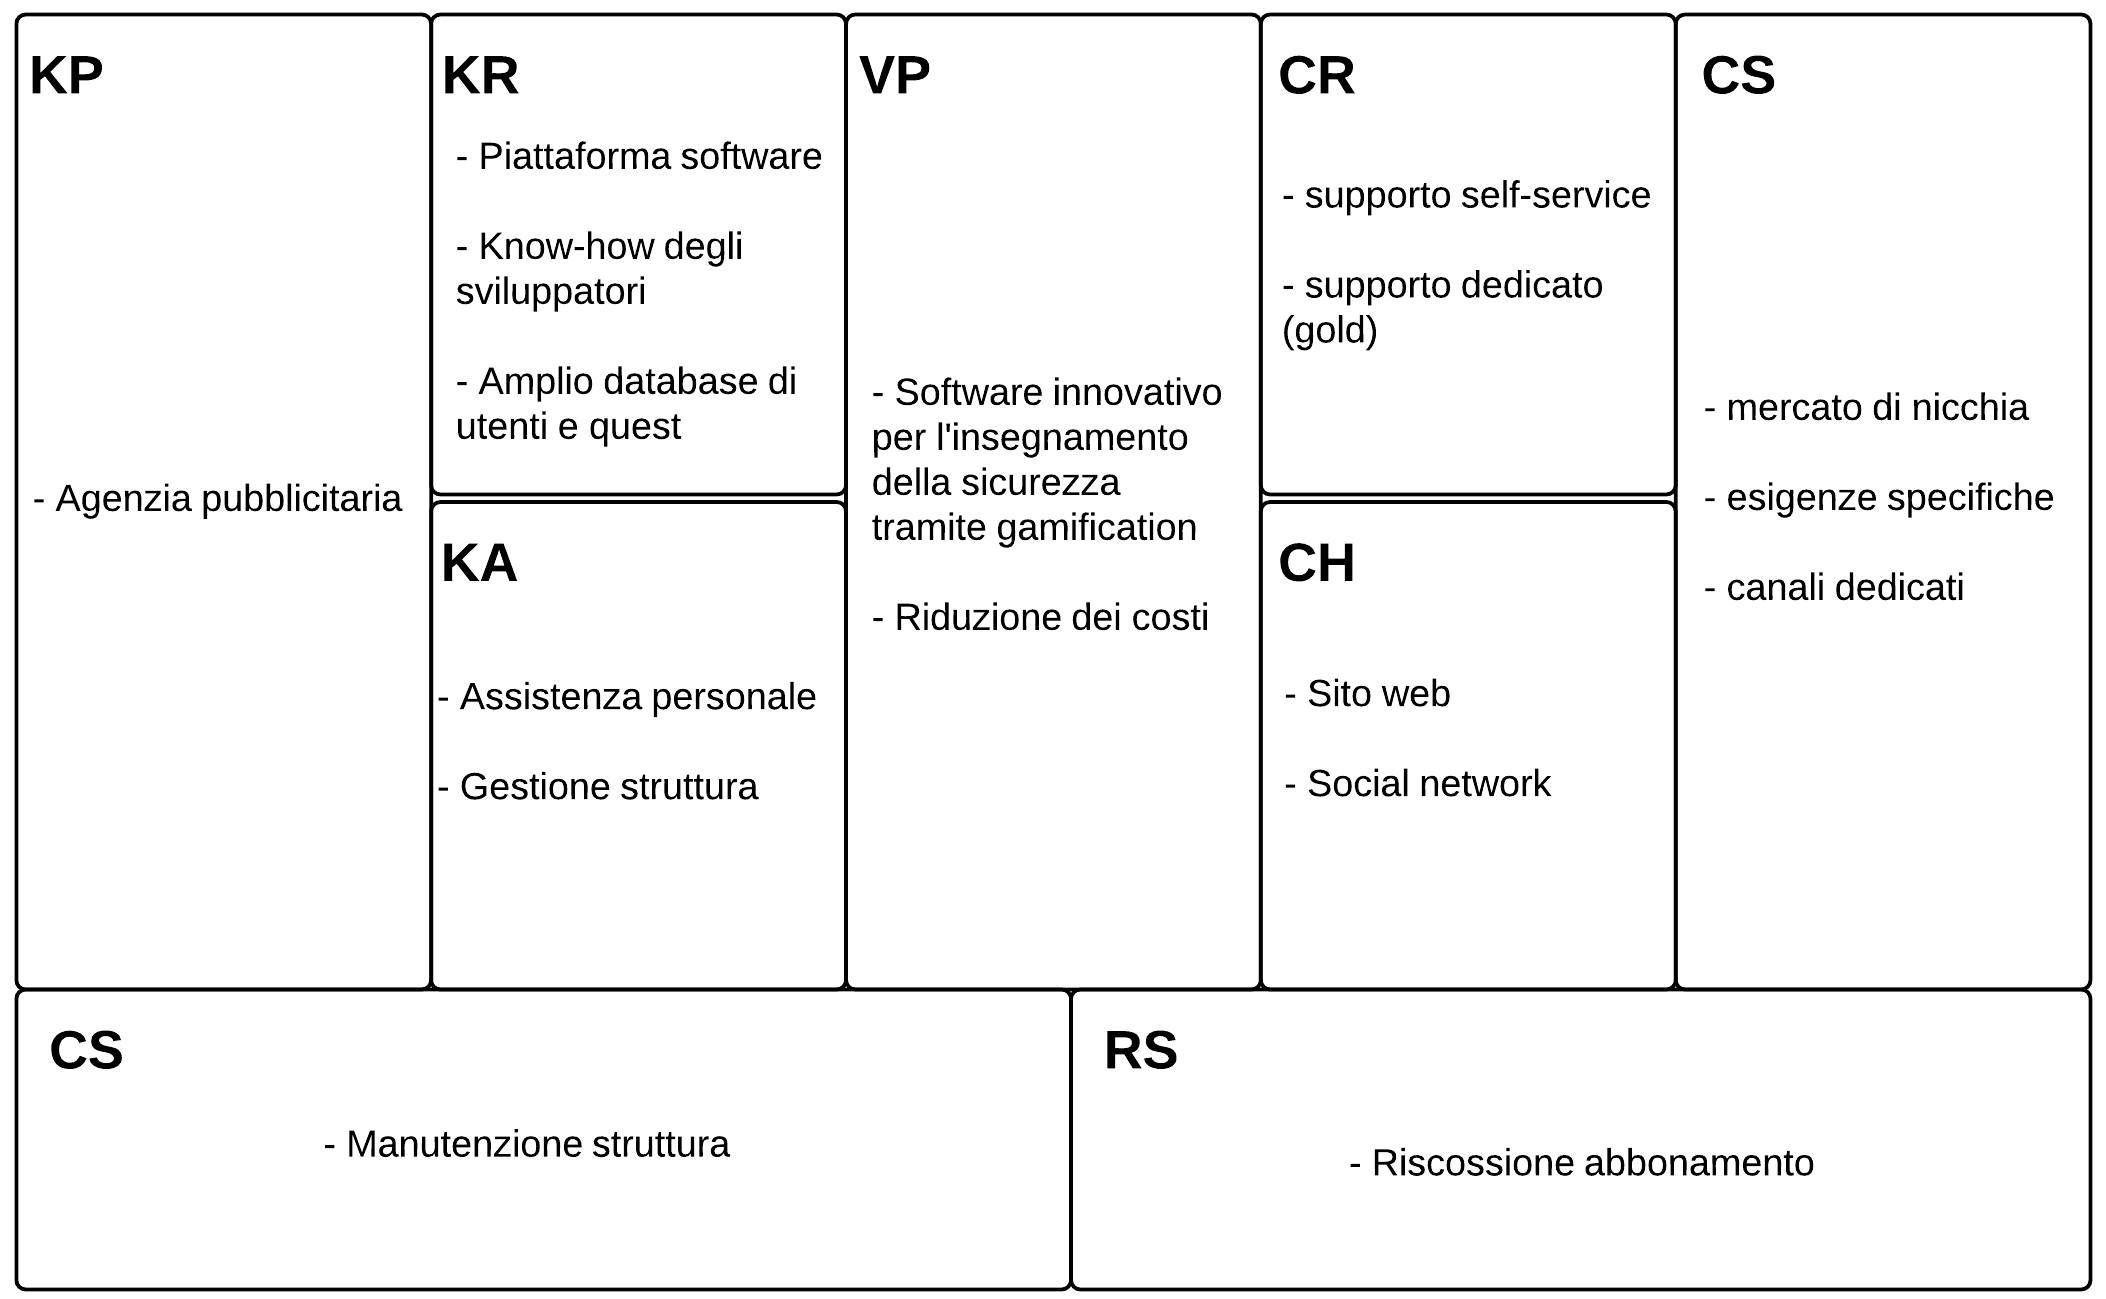
\includegraphics[scale=0.8]{images/BM.png}
\caption{Business model canvas}
\end{figure}



\end{document}
